\documentclass[11pt,letterpaper]{article}

\usepackage[utf8]{inputenc}
\usepackage[T1]{fontenc}
\usepackage[spanish]{babel}
\usepackage{graphicx}
\usepackage{geometry}
\usepackage{amsmath}
\usepackage{listings}
\usepackage{xcolor}
\usepackage{float}
\usepackage[hidelinks]{hyperref}

\geometry{letterpaper, margin=2.1cm}

\lstset{
    language=Python,
    basicstyle=\ttfamily\footnotesize,
    keywordstyle=\color{blue},
    commentstyle=\color{gray},
    stringstyle=\color{red!60!black},
    numbers=left,
    numberstyle=\tiny,
    frame=single,
    breaklines=true,
    showstringspaces=false,
    columns=fullflexible
}

\title{Taller 2: Histogramas de Imágenes Digitales}
\author{Camilo Eduardo Muñoz Albornoz\\
Procesamiento Digital de Imágenes\\
Universidad Tecnológica de Pereira}
\date{}

\begin{document}

\maketitle

\begin{center}
\textbf{Código fuente en GitHub}\\[0.2cm]
\textbf{Cuaderno o programa Python: }\href
{https://github.com/CamiloMunozAL/ProcDImagenes/blob/main/taller2/taller2.ipynb}
{\textcolor{blue}{\underline{\texttt{github.com/CamiloMunozAL/ProcDImagenes/blob/main/taller2/taller2.ipynb}}}}\\[0.15cm]
\textbf{Carpeta del Taller 2: }\href
{https://github.com/CamiloMunozAL/ProcDImagenes/tree/main/taller2}
{\textcolor{blue}{\underline{\texttt{github.com/CamiloMunozAL/ProcDImagenes/tree/main/taller2}}}}
\end{center}

\begin{abstract}
En este taller se implementó el cálculo de histogramas para imágenes en escala de grises y a color utilizando Python y OpenCV. Se emplearon dos estrategias: funciones proporcionadas por OpenCV y construcción manual del histograma mediante el recorrido de los píxeles de la imagen. Los resultados permitieron comprobar la relación entre los niveles de intensidad y su frecuencia, así como analizar independientemente los canales azul, verde y rojo de una imagen a color.
\end{abstract}

\section{Objetivos y preguntas del taller}

El objetivo general fue implementar y comprender el funcionamiento de los histogramas de imágenes digitales, tanto en escala de grises como a color. El informe responde, punto a punto, las cinco preguntas planteadas:

\begin{enumerate}
    \item Leer una imagen en escala de grises y producir su histograma.
    \item Cargar una imagen a color y producir el histograma de sus canales azul, verde y rojo.
    \item Construir mediante ciclos un vector de 256 posiciones con las frecuencias de una imagen en escala de grises.
    \item Graficar el histograma utilizando el vector construido manualmente.
    \item Repetir los puntos 3 y 4 para cada canal de una imagen a color.
\end{enumerate}

En todos los puntos se verificó que la suma de las frecuencias coincidiera con la cantidad de píxeles procesados.

\section{Imágenes utilizadas}

La imagen de entrada utilizada en los ejercicios fue \texttt{paisaje.png}. Para los histogramas en escala de grises se cargó con la opción \texttt{cv2.IMREAD\_GRAYSCALE}; para los histogramas de color se cargó conservando sus tres canales BGR. La Figura~\ref{fig:imagenes-entrada} presenta ambas representaciones.

\begin{figure}[H]
    \centering
    \begin{minipage}{0.47\textwidth}
        \centering
        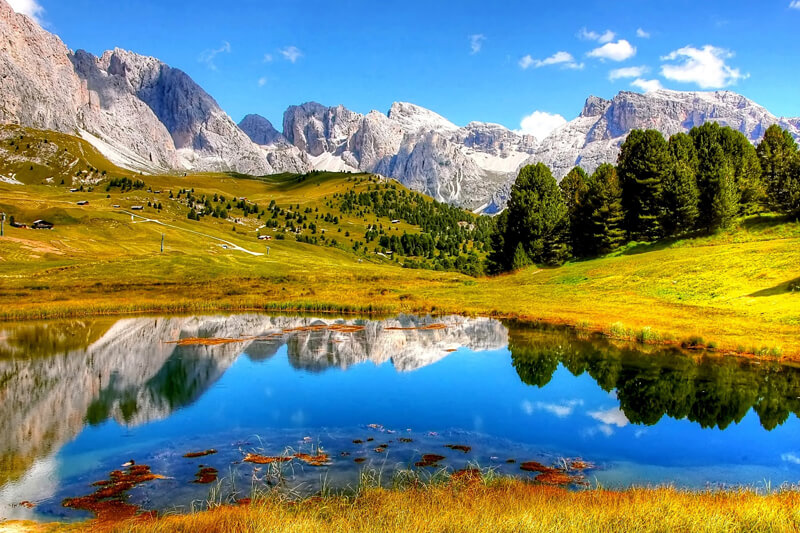
\includegraphics[width=\textwidth]{../images/paisaje.png}
        \textbf{(a)} Imagen a color
    \end{minipage}
    \hfill
    \begin{minipage}{0.47\textwidth}
        \centering
        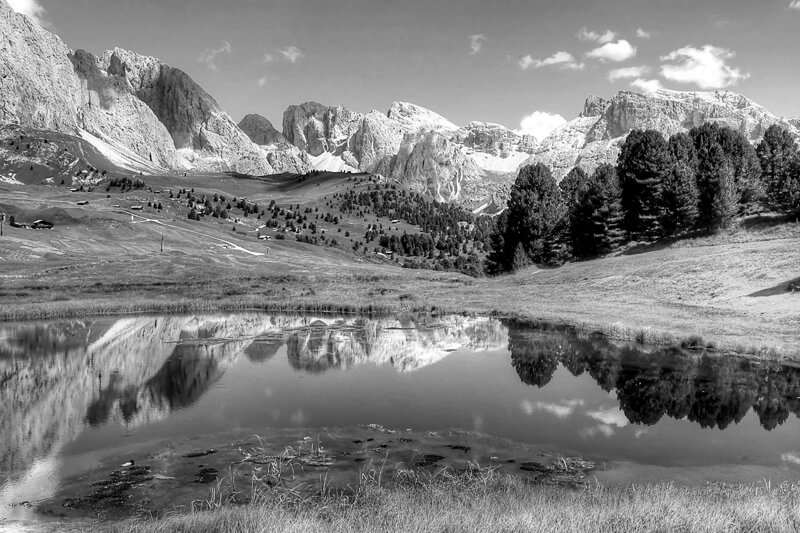
\includegraphics[width=\textwidth]{../../tallerBlancoNegro/resultados/paisaje_gris.png}
        \textbf{(b)} Imagen en escala de grises
    \end{minipage}
    \caption{Imágenes utilizadas como entrada para el análisis.}
    \label{fig:imagenes-entrada}
\end{figure}

\section{Fundamento y consideraciones}

Una imagen digital en escala de grises puede representarse mediante una matriz en la cual cada posición corresponde a un píxel. Para imágenes de 8 bits, cada píxel puede tomar valores entre 0 y 255, donde 0 representa negro, 255 blanco y los valores intermedios diferentes niveles de gris.

El histograma de una imagen representa la cantidad de píxeles existentes para cada nivel de intensidad. Puede expresarse como:

\begin{equation}
H(k)=\#\{(i,j): I(i,j)=k\}
\end{equation}

donde $k$ representa una intensidad entre 0 y 255 e $I(i,j)$ representa el valor del píxel ubicado en la fila $i$ y columna $j$.

Por tanto, la suma de todas las frecuencias debe ser igual a la cantidad total de píxeles:

\begin{equation}
\sum_{k=0}^{255} H(k) = M \times N
\end{equation}

donde $M$ y $N$ corresponden al alto y ancho de la imagen.

En una imagen a color cada píxel contiene tres componentes. Aunque normalmente se habla del modelo RGB, OpenCV carga las imágenes en orden BGR:

\begin{equation}
P(i,j)=[B,G,R]
\end{equation}

Por esta razón se puede construir un histograma independiente para cada canal. Es importante señalar que un histograma de color representa la distribución de intensidades de cada componente y no directamente la cantidad de píxeles de un determinado color.

\section{Desarrollo punto a punto}

\subsection{Punto 1: Histograma en escala de grises con OpenCV}

\textbf{Qué se hizo.} La imagen fue cargada directamente en escala de grises utilizando \texttt{cv2.imread}. Posteriormente se utilizó \texttt{cv2.calcHist}, indicando 256 niveles de intensidad en el intervalo de 0 a 256.

El fragmento principal utilizado fue:

\begin{lstlisting}
imagen_gris = cv2.imread(
    "images/paisaje.png",
    cv2.IMREAD_GRAYSCALE
)

histograma = cv2.calcHist(
    [imagen_gris],
    [0],
    None,
    [256],
    [0, 256]
)
\end{lstlisting}

La imagen utilizada presentó dimensiones de:

\begin{equation}
533 \times 800
\end{equation}

por lo que contiene:

\begin{equation}
533 \times 800 = 426400
\end{equation}

píxeles.

\textbf{Resultado.} La suma obtenida en el histograma fue igualmente de 426400, confirmando que todos los píxeles fueron contabilizados.

\begin{figure}[H]
    \centering
    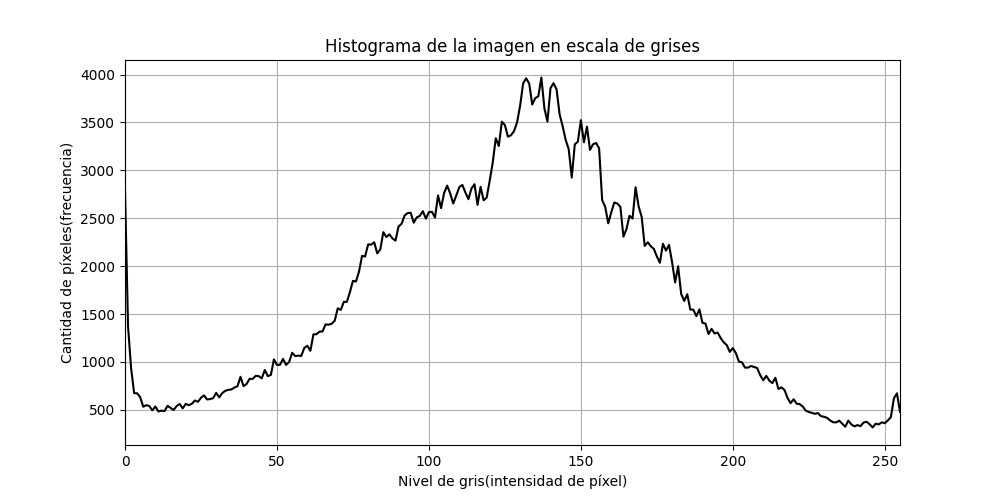
\includegraphics[width=\columnwidth]{../resultados/histogramapt1.png}
    \caption{Histograma de la imagen en escala de grises obtenido con OpenCV.}
    \label{fig:gris-opencv}
\end{figure}

\subsection{Punto 2: Histograma de los canales de color con OpenCV}

\textbf{Qué se hizo.} Para la imagen a color se calculó un histograma independiente para los canales azul, verde y rojo.

\begin{lstlisting}
canales = {
    0: "Blue",
    1: "Green",
    2: "Red"
}

for indice, color in canales.items():

    histograma_color = cv2.calcHist(
        [imagen_color],
        [indice],
        None,
        [256],
        [0, 256]
    )

    plt.plot(
        histograma_color,
        color=color.lower()
    )
\end{lstlisting}

La imagen presentó dimensiones:

\begin{equation}
533 \times 800 \times 3
\end{equation}

por lo que existen 426400 píxeles y 1279200 valores individuales almacenados entre los tres canales.

\textbf{Resultado.} Cada histograma presentó una suma de 426400:

\begin{itemize}
    \item Canal azul: 426400.
    \item Canal verde: 426400.
    \item Canal rojo: 426400.
\end{itemize}

Esto ocurre porque cada uno de los 426400 píxeles posee exactamente un valor azul, uno verde y uno rojo.

\begin{figure}[H]
    \centering
    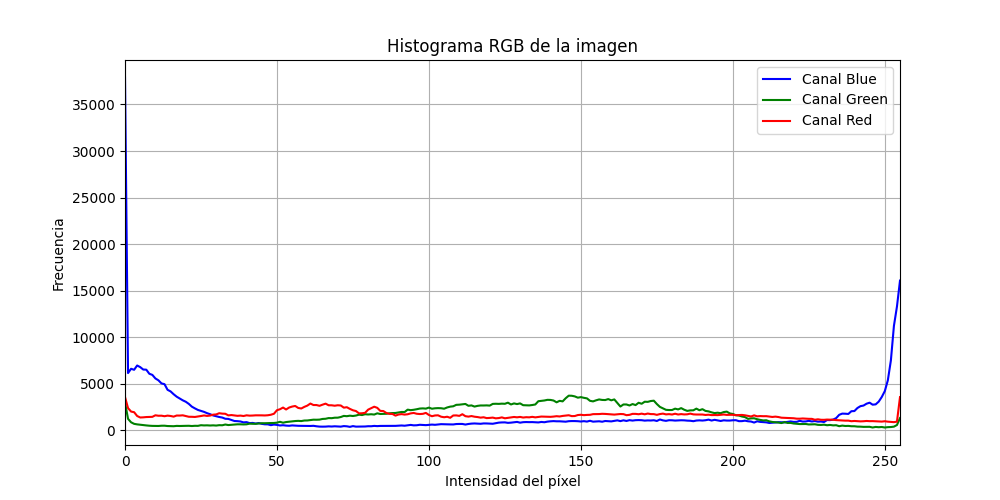
\includegraphics[width=\columnwidth]{../resultados/histogramacolorpt2.png}
    \caption{Histogramas de los canales azul, verde y rojo obtenidos con OpenCV.}
    \label{fig:rgb-opencv}
\end{figure}

\subsection{Punto 3: Construcción manual del vector en escala de grises}

\textbf{Qué se hizo.} Para comprender el funcionamiento interno del histograma se creó manualmente un vector de 256 posiciones y se recorrieron las filas y columnas de la imagen:

\begin{lstlisting}
histograma = [0] * 256

filas, columnas = imagen.shape

for i in range(filas):
    for j in range(columnas):
        nivel_gris = int(imagen[i, j])
        histograma[nivel_gris] += 1
\end{lstlisting}

Cada posición del vector corresponde a un nivel de gris. Por ejemplo, si un píxel posee intensidad 100, se incrementa la posición:

\begin{lstlisting}
histograma[100] += 1
\end{lstlisting}

De esta forma se recorrieron los 426400 píxeles de la imagen. Si un píxel posee intensidad 100, se incrementa la posición \texttt{histograma[100]}. Al finalizar, la suma del vector fue también de 426400, demostrando que cada píxel fue contado exactamente una vez.

\subsection{Punto 4: Histograma del vector manual}

\textbf{Qué se hizo.} Se utilizó el vector de frecuencias construido en el punto anterior para graficar los 256 niveles de gris. La posición del vector se ubicó en el eje horizontal y su frecuencia en el eje vertical.

\begin{figure}[H]
    \centering
    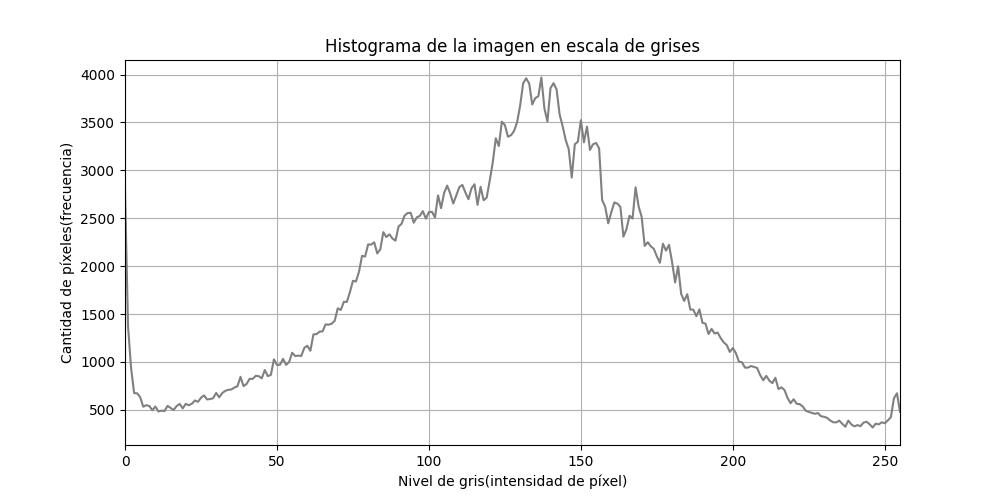
\includegraphics[width=\columnwidth]{../resultados/histogramapt3y4.png}
    \caption{Histograma construido manualmente mediante ciclos.}
    \label{fig:gris-manual}
\end{figure}

\textbf{Resultado.} El histograma manual presenta la misma distribución que el obtenido mediante \texttt{cv2.calcHist}, lo que confirma que la función de OpenCV realiza conceptualmente el mismo proceso de conteo, aunque mediante una implementación optimizada.

\subsection{Punto 5: Histogramas manuales de los canales de color}

\textbf{Qué se hizo.} Finalmente se aplicó el mismo procedimiento a cada componente de una imagen a color. Se crearon tres vectores independientes:

\begin{lstlisting}
histograma_blue = [0] * 256
histograma_green = [0] * 256
histograma_red = [0] * 256
\end{lstlisting}

Luego se recorrieron todos los píxeles:

\begin{lstlisting}
for fila in range(filas):
    for columna in range(columnas):

        pixel = imagen_color[fila, columna]

        histograma_blue[pixel[0]] += 1
        histograma_green[pixel[1]] += 1
        histograma_red[pixel[2]] += 1
\end{lstlisting}

Debido al formato BGR utilizado por OpenCV:

\begin{itemize}
    \item \texttt{pixel[0]} corresponde al azul.
    \item \texttt{pixel[1]} corresponde al verde.
    \item \texttt{pixel[2]} corresponde al rojo.
\end{itemize}

\begin{figure}[H]
    \centering
    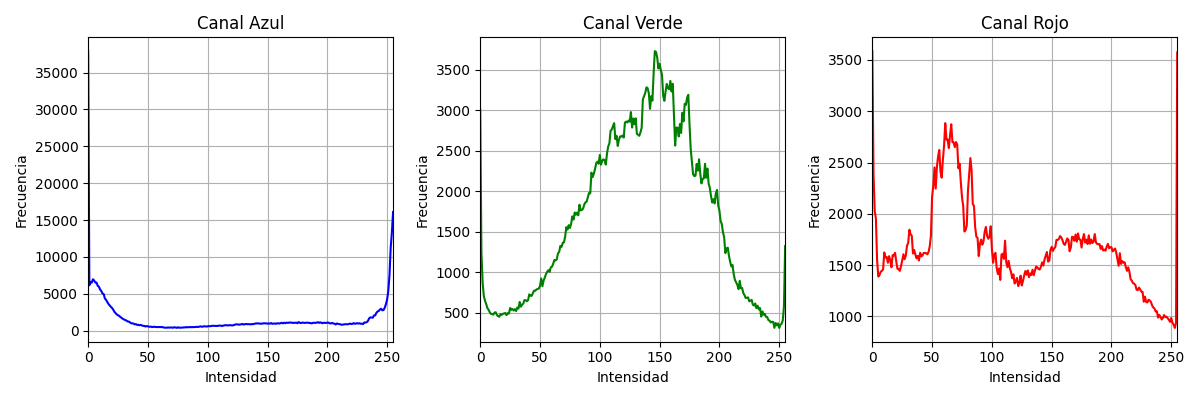
\includegraphics[width=\columnwidth]{../resultados/histogramas_horizontal.png}
    \caption{Histogramas manuales correspondientes a cada canal de color.}
    \label{fig:canales}
\end{figure}

También se representaron conjuntamente los tres histogramas para facilitar su comparación.

\begin{figure}[H]
    \centering
    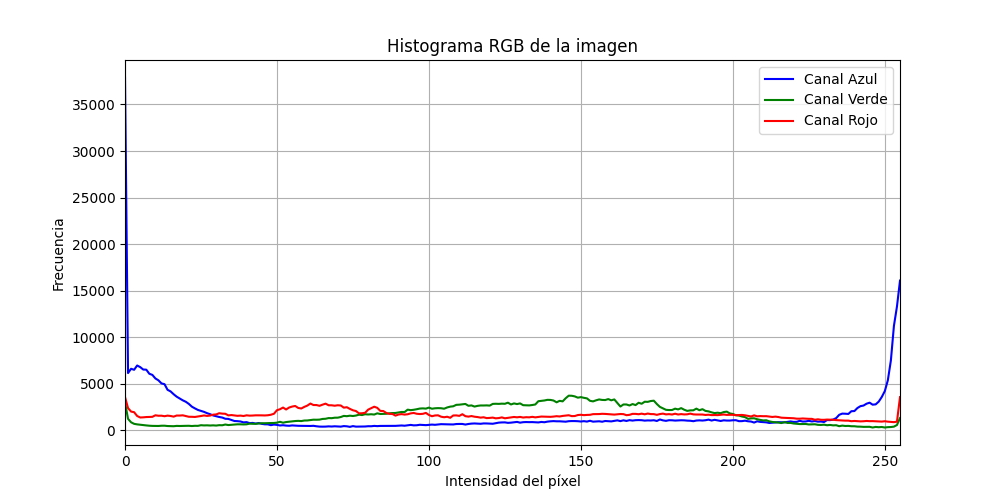
\includegraphics[width=\columnwidth]{../resultados/histogramacolorpt5.png}
    \caption{Comparación de los histogramas manuales de los tres canales.}
    \label{fig:rgb-manual}
\end{figure}

\section{Análisis de resultados}

Los histogramas obtenidos permiten observar la distribución de intensidades de la imagen utilizada.

En la imagen en escala de grises se observa una mayor concentración de píxeles aproximadamente entre los niveles 80 y 200. La mayor frecuencia se encuentra alrededor de las intensidades 130--150, donde se alcanzan valores próximos a 4000 píxeles por nivel. Esto indica una presencia importante de tonos medios.

También se presentan píxeles próximos a las intensidades 0 y 255, aunque en menor cantidad que los tonos intermedios. Por tanto, la imagen contiene regiones oscuras y claras además de una cantidad importante de tonos medios.

En los histogramas de color se observan comportamientos diferentes para cada canal. El canal azul presenta una concentración considerable en los extremos del rango. Particularmente, la intensidad azul 0 posee una frecuencia muy elevada, cercana a 35000 píxeles, mientras que también aparece una concentración importante próxima a 255.

Una intensidad azul igual a cero no significa necesariamente que el píxel sea negro. Por ejemplo, un píxel:

\begin{equation}
[B,G,R]=[0,180,220]
\end{equation}

contribuye al nivel cero del histograma azul, aunque contiene cantidades importantes de verde y rojo. Por tanto, los histogramas RGB describen la intensidad individual de cada canal, pero no permiten determinar por sí solos el color completo de un píxel.

El canal verde presenta mayor concentración principalmente en valores intermedios, aproximadamente entre 100 y 190, lo cual es coherente con la presencia considerable de vegetación en la imagen.

El canal rojo presenta una distribución más extendida, con concentraciones importantes en intensidades medias y un incremento próximo a la intensidad máxima.

Una observación importante es que los histogramas obtenidos manualmente mantienen la misma forma que los calculados mediante OpenCV. Esto permite validar el algoritmo implementado mediante ciclos y comprender el procedimiento realizado internamente por las funciones de la biblioteca.

\section{Conclusiones}

El histograma constituye una representación sencilla pero útil de la distribución de intensidades de una imagen digital. Para una imagen en escala de grises de 8 bits se requieren 256 posiciones, correspondientes a los posibles valores entre 0 y 255.

La implementación manual permitió comprobar que la construcción de un histograma consiste fundamentalmente en recorrer cada píxel y utilizar su intensidad como índice de un vector de frecuencias.

Los resultados obtenidos manualmente coincidieron con los generados mediante \texttt{cv2.calcHist}, validando la implementación realizada. En ambos casos, la suma de las frecuencias fue igual a los 426400 píxeles de la imagen.

En imágenes a color es necesario analizar independientemente los tres canales. Cada histograma contiene igualmente 426400 valores debido a que cada píxel aporta una intensidad a cada uno de los canales azul, verde y rojo.

Finalmente, se comprobó que un histograma RGB permite estudiar la distribución de cada componente de color, pero no conserva la relación espacial ni la combinación de los tres componentes de cada píxel. Por esta razón, el histograma permite caracterizar globalmente una imagen, pero no reconstruir su contenido visual únicamente a partir de sus frecuencias.

\end{document}